\documentclass[11pt]{article}
\usepackage[margin=1in]{geometry}
\usepackage[T1]{fontenc}
\usepackage{enumitem}
\usepackage{xurl}
\usepackage{hyperref}
\usepackage{longtable}
\usepackage{booktabs}
\usepackage{tikz}
\usepackage{graphicx}
\hypersetup{colorlinks=true,urlcolor=blue,linkcolor=blue}
\setlist{nosep,leftmargin=*}

\title{Midterm Project: Exploring AI Agent Tool Calling}
\author{Team project: two students per team}
\date{}
\begin{document}
\maketitle

\section{Project Overview}
Install and use \textbf{one} AI agent platform, either \textbf{Hermes Agent} or \textbf{OpenClaw}. Learn its main functions through hands-on tests, with particular attention to how the agent selects, invokes, and receives results from tools. Produce a high-level architecture diagram of the tool-calling mechanism and support the diagram with evidence from an actual agent run. Explain observed tool behavior; software for automatic graph generation is not required.

Work in a team of exactly two students. Both students must participate in installation, testing, analysis, reporting, and presentation. Teams receive the same project score when their documented contributions are substantially equal. The instructor may assign different individual scores when evidence shows unequal contributions.

\section{Learning Objectives}
By the end of the project, you should be able to:
\begin{enumerate}
  \item Install and configure Hermes Agent or OpenClaw with a working language model.
  \item Demonstrate basic agent functions and at least one actual tool call.
  \item Explain the path from a user question through model tool selection, tool execution, returned observation, and final response.
  \item Identify actual tool calls in run evidence and distinguish them from the agent's description of what it intended to do.
  \item Draw and defend a high-level architecture of the tool-calling mechanism.
\end{enumerate}

\section{Platform and Model Access}
Install and run your selected agent on the \textbf{University of Baltimore course VM}. Follow the instructor's VM access and setup instructions. Choose one of these model-access options:
\begin{enumerate}
  \item \textbf{Course-provided model:} connect the agent on the VM to the small model provided by the university. This option requires no student purchase. Check whether the model performs the tool calls needed for your tests, and document any limitations you observe.
  \item \textbf{Student-provided hosted API (optional):} connect the agent on the VM to a supported model provider using an API key you obtain yourself. A hosted model may respond faster or perform tool-use tasks better than the small course model, but this is not guaranteed. You are responsible for any charges; set a spending limit and use small test tasks. This option receives no extra credit.
\end{enumerate}
\textbf{Buying API tokens is not required.} Students using the course-provided model are evaluated by the same rubric. Do not include keys or tokens in the report, screenshots, slides, or GitHub repository. Use environment variables or a local configuration file excluded from Git, and remove your key from the shared VM when finished. Record the platform version or commit, VM environment, model/provider and version, installation method, and tool settings so another student can reproduce your work.

\section{Shared Starter Dataset and Questions}
Use the synthetic files and \textbf{midterm questions M0--M2} in \path{STARTER.md}. Copy the data folder identified there to your controlled VM workspace and give the agent read access. Run M0, M1, and M2 at least once using their supplied wording; replace \texttt{DATA\_DIR} with your actual path. M3 is a suggested missing-record limitation case. Save the original prompts and observed call evidence. The guide provides expected factual answers, but it does not prescribe a tool-call sequence: report the calls that actually occurred. Document any changed prompt and its reason, especially if the small course model does not invoke a tool on the first attempt.

\section{Required Work}
\subsection{Install and verify}
Follow the official installation/onboarding instructions for Hermes or OpenClaw. Show that the agent starts, connects to the selected model, and answers a simple question. Document the steps you actually performed, relevant commands or UI settings, and any problems you solved. Redact private paths, addresses, and credentials from shared evidence.

\subsection{Explore functions and test tools}
Explore at least \textbf{three} functions or capabilities of your chosen agent. These may include interactive chat, tool listing or policy configuration, file access, command execution in a controlled workspace, web retrieval, session history, or built-in activity/trace views. At least \textbf{one} test must show an actual tool invocation in a run record or other direct evidence. The same tool may be called more than once; different tool types are not required. Use only course-approved or your own test data and a disposable workspace for commands or file operations.

Run at least \textbf{three distinct prompts or tasks}: (a) a basic model-response check, (b) a task that causes at least one tool call, and (c) a cross-file task in which you explain the tool calls that actually occurred. Multiple calls are useful to observe but are not required for the midterm. If the agent declines or fails to call a tool, record that result, explain why it may have happened, adjust the prompt or tool configuration, and run a further test. For each task, save the exact prompt, relevant settings, agent response, and evidence of what the agent actually did. Include at least one controlled case that shows a tool error, denied action, or other limitation if it can be produced safely.

\subsection{Explain tool calling}
Identify the main components of the mechanism for your installed version: user interface or gateway, conversation/context, model request and tool definitions, model-selected call, policy or permission check (if present), tool executor, returned result, and final model response. Explain which component chooses a tool, which component executes it, and how the result returns to the model. Describe what you can observe directly and what remains an inference.

Draw a \textbf{high-level architecture diagram} with labeled components and arrows. Include the agent on the course VM, the chosen model (course-provided or hosted), at least one enabled tool, and the path for a returned tool result. Add a numbered call sequence for one real test question. Mark where request, execution, result, and call identity can be observed. The architecture may be drawn manually or with a diagram tool, but its labels must be readable in the PDF and slides. This is a conceptual architecture informed by documentation and observed runs; do not present unverified internal details as facts.

\noindent\textbf{Illustrative M1 sequence.} Figure~\ref{fig:midterm-example} shows how a question might lead to one file-tool call and a final answer. The model selects a tool, the agent runtime executes it, and the result returns to the model. Use evidence from your own run to describe what actually happened. This sequence is an example, not the high-level architecture diagram you must submit.

\begin{figure}[ht]
\centering
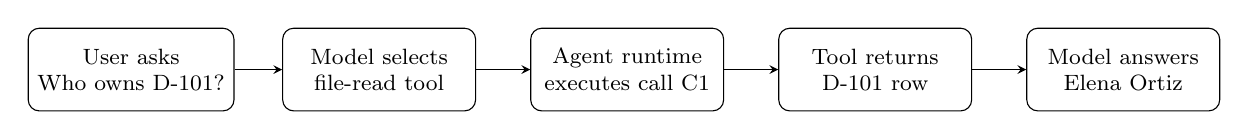
\begin{tikzpicture}[>=stealth,seqbox/.style={draw,rounded corners,minimum width=2.45cm,minimum height=1.05cm,align=center,font=\footnotesize}]
  \node[seqbox] (q) at (1.4,0) {User asks\\Who owns D-101?};
  \node[seqbox] (m) at (4.55,0) {Model selects\\file-read tool};
  \node[seqbox] (a) at (7.7,0) {Agent runtime\\executes call C1};
  \node[seqbox] (t) at (10.85,0) {Tool returns\\D-101 row};
  \node[seqbox] (r) at (14.0,0) {Model answers\\Elena Ortiz};
  \draw[->] (q) -- (m);
  \draw[->] (m) -- (a);
  \draw[->] (a) -- (t);
  \draw[->] (t) -- (r);
\end{tikzpicture}
\caption{One possible M1 tool-calling sequence. The actual tool name, call ID, and evidence must come from the team's run.}
\label{fig:midterm-example}
\end{figure}

\noindent\textbf{Hermes running example.} Figure~\ref{fig:hermes-tool-calls} shows part of a Hermes terminal session during a separate task. The highlighted lines show a process poll and wait, then a terminal command followed by another wait. This illustrates that one task may involve several tool invocations. The screenshot is only a partial view: it does not establish every call's arguments, result, or complete order. For your own test, use the available run record to identify and explain the calls you actually observed.

\begin{figure}[htbp]
\centering
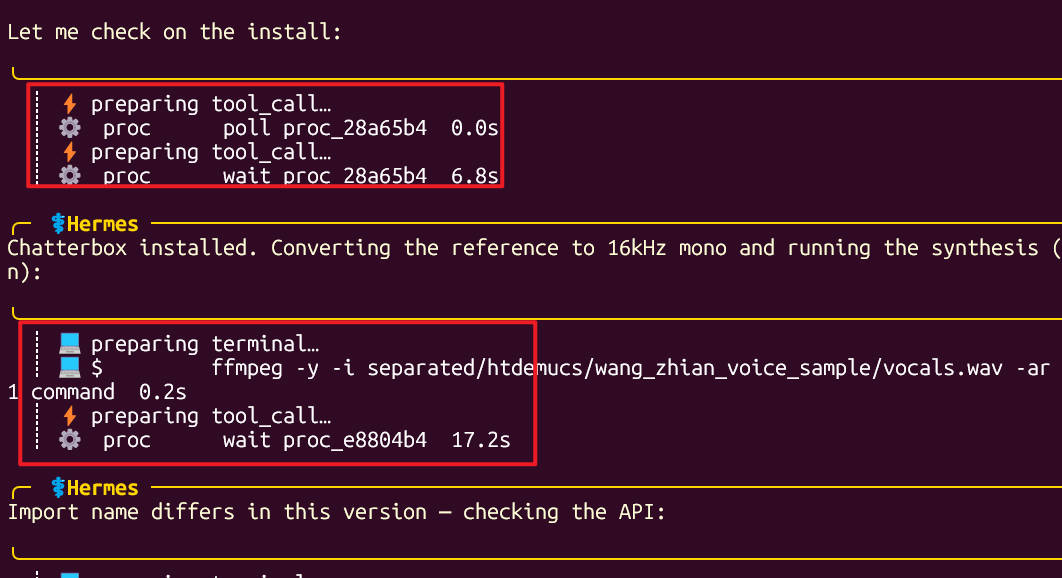
\includegraphics[width=\linewidth]{tool_calling_hermes.jpg}
\caption{Example Hermes session showing visible tool-call activity. The highlighted status lines and terminal command are from an illustrative task, not the required M1 dataset question.}
\label{fig:hermes-tool-calls}
\end{figure}

\subsection{Assess observation limits}
Identify one way to inspect tool-call evidence in your selected platform (for example, Hermes hooks or OpenClaw trajectory/audit records). State what it records, one visibility gap, and one question you could not resolve from the available evidence. Implementing a separate collector is not required.

\section{IEEE-Style Midterm Report in Overleaf}
Create the report in Overleaf using the official \textbf{IEEE Conference Template}: \url{https://www.overleaf.com/latex/templates/ieee-conference-template/grfzhhncsfqn}. Click ``Open as Template'' to make the team's copy. Use its two-column \texttt{IEEEtran} conference format and numbered references. Aim for \textbf{4--6 pages of main text}, excluding references and an optional appendix. Include:
\begin{enumerate}
  \item \textbf{Title, authors, abstract, and keywords}: platform, model access path, tests, and main finding.
  \item \textbf{I. Introduction}: purpose, scope, and team objectives.
  \item \textbf{II. Platform and Setup}: agent version, system/VM, model/provider, installation and verification steps.
  \item \textbf{III. Tool-Calling Architecture}: labeled high-level diagram, component roles, and numbered sequence for one real question.
  \item \textbf{IV. Test Method}: exact prompts, enabled tools, expected observations, and evidence source.
  \item \textbf{V. Results}: per-task table of actual behavior, tool names and outcomes, representative evidence, and discrepancies.
  \item \textbf{VI. Discussion and Limitations}: visibility gaps, unresolved questions, and how evidence could be improved.
  \item \textbf{VII. Conclusion}: what the team learned and what remains unresolved.
  \item \textbf{References}: IEEE-style numbered citations to platform and model documentation and other sources.
  \item \textbf{Appendix (optional)}: additional redacted screenshots, command output, and detailed setup notes.
\end{enumerate}
Include the team's \textbf{GitHub repository URL} and evaluated commit hash in the report. Include a short \textbf{team contributions and AI-assistance statement} identifying each student's work, any ChatGPT/Claude or other AI help, and how outputs were checked. AI assistance is encouraged, but the team must verify and understand all submitted material.

\section{Deliverables and Submission}
Each team must create a \textbf{GitHub repository} containing setup/reproduction instructions, a copy of the shared synthetic data, safe configuration examples, prompts, redacted run evidence, the architecture diagram source or image, and any test scripts. Make the repository accessible to the instructor by the deadline. Do not commit credentials, private data, or unrestricted logs that may contain them.

Each student must independently submit \textbf{one Canvas submission} containing:
\begin{enumerate}
  \item The same team midterm report PDF in IEEE format.
  \item A share link to the editable Overleaf project with instructor access.
  \item The team's presentation slides (PPT or PPTX).
  \item The team's GitHub repository link and evaluated commit hash.
  \item A short individual contribution statement, consistent with the team report.
\end{enumerate}
Both students must participate in the \textbf{oral presentation}. Demonstrate installation/model connection, one tool-using run, and the architecture diagram. A recorded backup may be used if the live model or VM is unavailable. Follow the instructor's Canvas announcement for the due date, presentation length, VM access details, and submission link.

\section{Evaluation Rubric (100 Points)}
\renewcommand{\arraystretch}{1.15}
\begin{longtable}{p{0.29\linewidth}p{0.56\linewidth}r}
  \toprule
  Criterion                         & Evidence expected                                                                                                                                           & Points       \\
  \midrule
  \endhead
  Installation and model connection & Correct agent installation, documented version/environment/model, working connection, and reproducible verification.                                        & 20           \\
  Function exploration              & At least three capabilities explored, including one actual tool invocation; clear explanation of configuration and behavior.                                 & 15           \\
  Tool-use tests and evidence       & Three distinct tasks, including tool use and cross-file interpretation; exact prompts, observed calls, results, and a documented error or limitation where feasible. & 20           \\
  Tool-calling architecture         & Accurate labeled diagram, component responsibilities, tool/result path, numbered real call sequence, and observation versus inference.                      & 20           \\
  IEEE report and repository        & IEEE structure and citations, clear results, GitHub link/commit, reproducibility, safe evidence, and contribution/AI-use disclosure.                        & 15           \\
  Presentation and participation    & Both students present, demonstrate a tool call, explain the diagram, and document substantially equal contributions.                                        & 10           \\
  \midrule
  \textbf{Total}                    &                                                                                                                                                             & \textbf{100} \\
  \bottomrule
\end{longtable}

A failed or refused tool call can earn credit when documented and analyzed. Invented evidence of successful tool use cannot.

\section{Official Starting Points}
\begin{enumerate}
  \item Nous Research, ``Hermes Agent Quickstart,'' \url{https://github.com/NousResearch/hermes-agent/blob/main/website/docs/getting-started/quickstart.md}.
  \item Nous Research, ``Hermes Agent: Hooks,'' \url{https://github.com/NousResearch/hermes-agent/blob/main/website/docs/user-guide/features/hooks.md}.
  \item OpenClaw, ``Onboarding (CLI),'' \url{https://docs.openclaw.ai/start/wizard}.
  \item OpenClaw, ``Tools overview,'' \url{https://docs.openclaw.ai/tools}.
  \item OpenClaw, ``Local models,'' \url{https://docs.openclaw.ai/gateway/local-models}.
  \item OpenClaw, ``Trajectory bundles,'' \url{https://docs.openclaw.ai/tools/trajectory}.
  \item IEEE, ``Conference template,'' \url{https://www.overleaf.com/latex/templates/ieee-conference-template/grfzhhncsfqn}.
\end{enumerate}
Use the instructions that match the version you install; agent commands and model support may change.

\end{document}
